\chapter{Membraanverkeer en het sorteren van eiwitten}\label{ch:b3:membrane-traffic}

Een cel van de alvleesklier maakt zo'n tien miljoen moleculen
verteringsenzym per minuut, verpakt ze in korrels en laat ze op een
signaal uit de darm los in een afvoerbuis --- zonder ooit één molecuul
trypsine in haar eigen cytoplasma vrij te laten. Een levercel haalt
cholesterol uit het bloed door de deeltjes die het dragen in hun geheel
te verzwelgen, duizenden per minuut, en brengt elke receptor terug naar
het oppervlak voor de volgende. Een pas gemaakt eiwit dat voor het
mitochondrion, de kern, het \omterm{def:b3:membrane-traffic:endocytosis}{lysosoom}, het membraan of de buitenwereld
bestemd is bereikt zijn adres tussen een tiental compartimenten met een
foutenpercentage waar een postdienst zich voor zou schamen. Dit
hoofdstuk gaat over dat sorteren: de signalen die in eiwitten zijn
geschreven, de machines die ze lezen, de blaasjes die membraan en
vracht tussen compartimenten vervoeren, de manteleiwitten die de
blaasjes vorm geven en de eiwitten die ze met het juiste doelwit laten
versmelten, en het verkeer in twee richtingen --- secretie naar buiten,
endocytose naar binnen --- dat een eukaryote cel elke seconde van haar
leven volhoudt.

\section{Signalen en adressen}

\begin{definition}[Sorteersignalen]\label{def:b3:membrane-traffic:signals}
\index{sorteersignaal}\index{signaalpeptide}\index{kernlokalisatiesignaal}\index{presequentie}
Een \emph{sorteersignaal} is een segment van een eiwit, of een
wijziging daarvan, dat wordt gelezen door een receptor die het eiwit
naar één compartiment brengt. Het \emph{signaalpeptide}, een stuk van
\numrange{15}{30} residuen aan de aminoterminus met een hydrofobe kern,
stuurt een eiwit tijdens het maken het endoplasmatisch reticulum in;
van daaruit leidt de standaardroute via het golgiapparaat naar het
plasmamembraan of naar buiten, en verdere signalen leiden het af naar
het \omterm{def:b3:membrane-traffic:endocytosis}{lysosoom} (een gefosforyleerde suiker) of terug naar het reticulum
(de carboxyterminale sequentie KDEL). Een
\emph{kernlokalisatiesignaal}, een korte basische plek zoals PKKKRKV,
wordt gebonden door importines die het gevouwen eiwit door de kernporie
dragen; een mitochondriale \emph{presequentie}, een amfipathische helix
van \numrange{20}{50} residuen, wordt herkend door receptoren op het
buitenmembraan en ongevouwen door translocasen van beide membranen
geregen; peroxisomale enzymen eindigen op SKL. Eiwitten zonder een van
deze signalen blijven in het cytosol. Elk signaal is op dezelfde wijze
gevonden: het weghalen laat het eiwit in het cytosol, het aan een
cytosolisch eiwit enten stuurt dat eiwit naar het compartiment.
\end{definition}

\begin{proof}[Bewijsmateriaal]
Blobel en Dobberstein (1975) vertaalden het boodschapper-RNA van een
lichte keten van een antilichaam in een celvrij systeem. Zonder
membranen was het product ongeveer twintig residuen langer dan het
uitgescheiden eiwit; met fragmenten van endoplasmatisch reticulum
\emph{tijdens} de translatie toegevoegd had het product de
uitgescheiden grootte en was het beschermd tegen toegevoegd protease
--- het zat in de blaasjes --- terwijl membranen die na de translatie
werden toegevoegd niets deden. Het extra aminoterminale segment, het
\omterm{def:b3:membrane-traffic:signals}{signaalpeptide}, is nodig om het reticulum binnen te komen, wordt
daarbinnen verwijderd en werkt alleen zolang de keten wordt gemaakt: de
\emph{signaalhypothese}, tot in elk detail bevestigd toen de receptor
(het signaalherkenningsdeeltje, Walter en Blobel 1981) en het kanaal
(Sec61) waren gezuiverd.
\end{proof}

\begin{omfigure}
\begin{tikzpicture}[every node/.style={font=\scriptsize}, >=stealth]
  % ER membrane
  \fill[omDef!15] (0,0) rectangle (12,-1.6);
  \draw[very thick, omDef] (0,0) -- (12,0); \draw[very thick, omDef] (0,-0.35) -- (12,-0.35);
  \node[right, omDef!70!black] at (0.1,-1.3) {lumen van het ER};
  \node[right] at (0.1,2.9) {cytosol};
  % stage 1: ribosome with emerging signal peptide + SRP
  \draw[thick, fill=gray!25] (1.4,1.6) circle (0.5); \draw[thick, fill=gray!25] (1.4,0.95) ellipse (0.62 and 0.3);
  \draw[very thick, omThm] (1.4,0.65) -- (1.4,0.2) -- (1.9,0.1);
  \draw[thick, fill=omProp!40] (2.1,0.35) ellipse (0.35 and 0.2); \node[above right] at (2.2,0.5) {SRP};
  \node[below, align=center] at (1.7,-1.7) {1. het signaalpeptide komt naar buiten;\\SRP bindt, de translatie pauzeert};
  % stage 2: docking at SRP receptor and translocon
  \draw[->, thick] (3.2,1.2) -- (4.2,1.2);
  \draw[thick, fill=gray!25] (5.6,1.75) circle (0.5); \draw[thick, fill=gray!25] (5.6,1.1) ellipse (0.62 and 0.3);
  \draw[thick, fill=omMeth!40] (5.2,0.0) rectangle (5.45,-0.35); \draw[thick, fill=omMeth!40] (5.75,0.0) rectangle (6.0,-0.35);
  \node[below, align=center] at (5.9,-1.7) {2. de SRP-receptor dokt het\\aan Sec61; SRP vertrekt};
  \draw[very thick, omThm] (5.6,0.8) -- (5.6,-0.2);
  \draw[thick, fill=omProp!40] (4.7,0.15) ellipse (0.3 and 0.18); \node[above] at (4.7,0.33) {SRP-receptor};
  % stage 3: translocation, cleavage, glycosylation
  \draw[->, thick] (7.2,1.2) -- (8.2,1.2);
  \draw[thick, fill=gray!25] (9.6,1.75) circle (0.5); \draw[thick, fill=gray!25] (9.6,1.1) ellipse (0.62 and 0.3);
  \draw[thick, fill=omMeth!40] (9.2,0.0) rectangle (9.45,-0.35); \draw[thick, fill=omMeth!40] (9.75,0.0) rectangle (10.0,-0.35);
  \draw[very thick, omThm] (9.6,0.8) -- (9.6,-0.5) .. controls (9.6,-1.0) and (10.3,-1.1) .. (10.6,-0.7);
  \draw[omThm, thick] (10.9,-0.9) -- (11.2,-0.9); \node[right, font=\tiny] at (11.0,-1.15) {signaal geknipt};
  \fill[omExo] (10.3,-1.0) circle (0.07); \fill[omExo] (10.45,-1.12) circle (0.07); \node[below, font=\tiny] at (10.2,-1.15) {suikers};
  \node[below, align=center] at (10.0,-1.7) {3. de keten steekt over terwijl zij wordt gemaakt;\\signaal geknipt, suikers toegevoegd};
\end{tikzpicture}

{\small De signaalhypothese. Een \omterm{def:b3:membrane-traffic:signals}{signaalpeptide} aan het begin van de
ontluikende keten wordt gebonden door het signaalherkenningsdeeltje,
dat de translatie pauzeert en het ribosoom aan het Sec61-kanaal dokt;
de keten steekt daarna het membraan over terwijl zij wordt gemaakt, het
signaal wordt in het lumen afgeknipt, en er worden suikers toegevoegd.}
\end{omfigure}

\begin{proposition}[Membraaneiwitten en topologie]\label{prop:b3:membrane-traffic:topology}
\index{stoptransfersequentie}\index{membraantopologie}
Een hydrofoob stuk van ongeveer twintig residuen midden in een keten
die wordt getransloceerd werkt als \emph{stoptransfersequentie}: het
kanaal gaat opzij open en laat het in de dubbellaag los als
transmembraanhelix, met het al getransloceerde deel in het lumen en de
rest in het cytosol gemaakt. Een tweede zo'n stuk hervat de
translocatie, en een eiwit met $n$ afwisselende signalen eindigt met
$n$ membraandoorspannende helices. De richting die in het reticulum
wordt vastgelegd verandert nooit meer: wat naar het lumen van het
reticulum wijst, wijst naar het lumen van het golgiapparaat en van elk
blaasje daarna, en na fusie met het plasmamembraan naar de
\emph{buitenkant} van de cel. Daarom zitten suikers, die alleen in het
lumen worden toegevoegd, altijd aan de extracellulaire kant van een
oppervlakte-eiwit, en is de topologie van een receptor af te lezen aan
de ligging van zijn glycosyleringsplaatsen.
\end{proposition}

\begin{method}[Pulsmerking en jacht]\label{met:b3:membrane-traffic:pulse-chase}
\index{pulsmerking}\index{autoradiografie}
Om een populatie pas gemaakte moleculen door de cel te volgen: (1)
stel de cellen kort bloot (de \emph{puls}, enkele minuten) aan een
radioactieve of anderszins gemerkte voorloper --- getritieerd leucine
voor eiwitten; (2) vervang die door een overmaat ongemerkte voorloper
(de \emph{jacht}), zodat er geen nieuw merkstof meer wordt ingebouwd;
(3) fixeer op gezette tijden monsters van cellen en lokaliseer het
merkstof met autoradiografie in elektronenmicroscopische opnamen, of
door de compartimenten te isoleren en te tellen; (4) zet het deel van
het merkstof in elk compartiment tegen de tijd uit. De volgorde waarin
de compartimenten vollopen en leeglopen is de route; de tijden geven de
verblijfstijd in elk. Het laboratorium van Palade (jaren zestig) paste
haar toe op de acinaire cel van de alvleesklier en vond het merkstof
na \qty{3}{min} in het ruwe reticulum, na \qty{20}{min} in het
golgiapparaat, na \qty{40}{min} in condenserende vacuolen en korrels,
en na een uur en op een signaal in de afvoerbuis: de secretieroute,
uitgezet in de tijd.
\end{method}

\begin{theorem}[Opeenvolgende compartimenten en de pulscurven]\label{thm:b3:membrane-traffic:pulse-chase}
\index{compartimentmodel}
Laat een puls gemerkt eiwit compartiment $A$ verlaten voor $B$ met
eerste-ordesnelheid $k_{1}$, en $B$ verlaten voor $C$ met snelheid
$k_{2}$, waarbij $C$ het vasthoudt. Met al het merkstof in $A$ op
$t = 0$ geldt
\[
A(t) = e^{-k_{1}t},\qquad
B(t) = \frac{k_{1}}{k_{2} - k_{1}}\bigl(e^{-k_{1}t} - e^{-k_{2}t}\bigr),
\qquad
C(t) = 1 - A - B,
\]
en bereikt het merkstof in $B$ een maximum op
$t^{*} = \ln(k_{2}/k_{1})/(k_{2} - k_{1})$. De gemiddelde verblijfstijd
in $A$ is $1/k_{1}$ en in $B$ is $1/k_{2}$, wat de volgorde van de twee
snelheden ook is.
\end{theorem}
\begin{proof}
$\mathrm{d}A/\mathrm{d}t = -k_{1}A$ geeft de exponentiële vorm. Voor
$B$ geldt
$\mathrm{d}B/\mathrm{d}t = k_{1}A - k_{2}B = k_{1}e^{-k_{1}t} - k_{2}B$;
probeer $B = \beta(e^{-k_{1}t} - e^{-k_{2}t})$: de afgeleide is
$\beta(-k_{1}e^{-k_{1}t} + k_{2}e^{-k_{2}t})$ en $-k_{2}B = \beta(-k_{2}
e^{-k_{1}t} + k_{2}e^{-k_{2}t})$, zodat de vergelijking $\beta(k_{2}
- k_{1})e^{-k_{1}t} = k_{1}e^{-k_{1}t}$ vergt, dus $\beta = k_{1}/(k_{2} -
k_{1})$, en $B(0) = 0$ zoals vereist. Stelt men $\mathrm{d}B/\mathrm{d}t =
0$, dan is $k_{1}e^{-k_{1}t} = k_{2}e^{-k_{2}t}$, waaruit $t^{*}$
volgt. De gemiddelde tijd die een molecuul doorbrengt in een
compartiment dat het met snelheid $k$ verlaat is $\int_{0}^{
\infty} t\,k e^{-kt}\,\mathrm{d}t = 1/k$.
\end{proof}

\begin{example}[De cel van Palade in getallen]\label{ex:b3:membrane-traffic:palade}
Neem $k_{1} = \qty{0.1}{min^{-1}}$ (tien minuten in het reticulum) en
$k_{2} = \qty{0.05}{min^{-1}}$ (twintig in het golgiapparaat). Het
golgiapparaat bereikt zijn maximum op
$t^{*} = \ln 2/0.05 = \qty{13.9}{min}$ en bevat dan $B = 2(e^{-1.39} -
e^{-0.69}) = 2(0.25 - 0.50)\cdot(-1) = 0.50$: de helft van het merkstof.
Na \qty{40}{min} is $A = 0.018$, $B = 2(0.018 - 0.135) \to 0.23$ en
$C = 0.75$: drie kwart van het eiwit heeft de korrels bereikt. De
waargenomen curven van het laboratorium van Palade hebben deze vorm, en
ze aanpassen was de eerste manier waarop de verblijfstijden werden
gemeten.
\end{example}

\begin{omfigure}
\begin{tikzpicture}
\begin{axis}[
  width=0.7\linewidth, height=5.6cm,
  axis x line=bottom, axis y line=left,
  xmin=0, xmax=80, ymin=0, ymax=1.05,
  xlabel={minuten na de puls}, ylabel={fractie van het merkstof},
  xlabel style={font=\small, at={(axis description cs:0.5,-0.12)}, anchor=north},
  ylabel style={font=\small},
  tick label style={font=\small}, xtick={0,20,40,60,80}, ytick={0,0.5,1},
  clip=false,
]
\addplot[very thick, omDef, domain=0:80, samples=80] {exp(-0.1*x)};
\addplot[very thick, omProp, domain=0:80, samples=80] {2*(exp(-0.05*x)-exp(-0.1*x))};
\addplot[very thick, omMeth!70!black, domain=0:80, samples=80] {1-exp(-0.1*x)-2*(exp(-0.05*x)-exp(-0.1*x))};
\node[font=\scriptsize, omDef, anchor=south west] at (axis cs:4,0.62) {reticulum, $A$};
\node[font=\scriptsize, omProp, anchor=south] at (axis cs:14,0.53) {golgiapparaat, $B$};
\node[font=\scriptsize, omMeth!70!black, anchor=north west] at (axis cs:45,0.72) {korrels, $C$};
\end{axis}
\end{tikzpicture}

{\small Pulscurven uit het tweesnelhedenmodel met $k_{1} =
\qty{0.1}{min^{-1}}$ en $k_{2} = \qty{0.05}{min^{-1}}$: het merkstof
verlaat het reticulum exponentieel, gaat door het golgiapparaat met een
maximum bij \qty{14}{min}, en hoopt zich op in de korrels.}
\end{omfigure}

\section{Het endoplasmatisch reticulum: vouwen, suikers en kwaliteit}

\begin{definition}[N-glycosylering en kwaliteitsbewaking]\label{def:b3:membrane-traffic:glycosylation}
\index{N-glycosylering}\index{calnexinecyclus}\index{ER-geassocieerde afbraak}\index{respons op ongevouwen eiwitten}
Zodra de keten het lumen binnenkomt wordt een vooraf samengesteld
oligosacharide van veertien suikers (twee N-acetylglucosamines, negen
mannoses, drie glucoses) van een lipidedrager overgezet op asparagines
in de sequentie Asn-X-Ser/Thr --- de \emph{N-glycosylering}. De drie
glucoses worden daarna een voor een weggeknipt, en dat knippen is een
vouwklok: een eiwit dat nog één glucose draagt wordt vastgehouden door
de \omterm{def:b3:structural-biology:chaperones}{chaperonne} calnexine; een eiwit waarvan de laatste glucose is
verwijderd maar dat nog niet is gevouwen wordt opnieuw geglucosyleerd
door een enzym dat blootliggende hydrofobe plekken herkent, en keert
terug naar calnexine --- de \emph{calnexinecyclus}. Eiwitten die
herhaaldelijk falen worden terug het cytosol in getrokken,
geubiquitineerd en door het proteasoom vernietigd: de
\emph{ER-geassocieerde afbraak} (ERAD). Wanneer ongevouwen eiwitten
zich sneller ophopen dan zij kunnen worden gevouwen of vernietigd,
starten sensoren in het reticulummembraan de \emph{respons op
ongevouwen eiwitten}: de translatie wordt vertraagd, chaperonnegenen
worden aangezet, het reticulum wordt uitgebreid, en als de stress
aanhoudt wordt de cel gedood. De meest voorkomende mutatie bij
taaislijmziekte ($\Delta$F508 in CFTR) maakt een kanaal dat zou werken
maar zich te traag vouwt, door ERAD wordt opgepakt en het oppervlak
nooit bereikt; geneesmiddelen die het helpen vouwen zijn nu een
behandeling.
\end{definition}

\begin{omfigure}
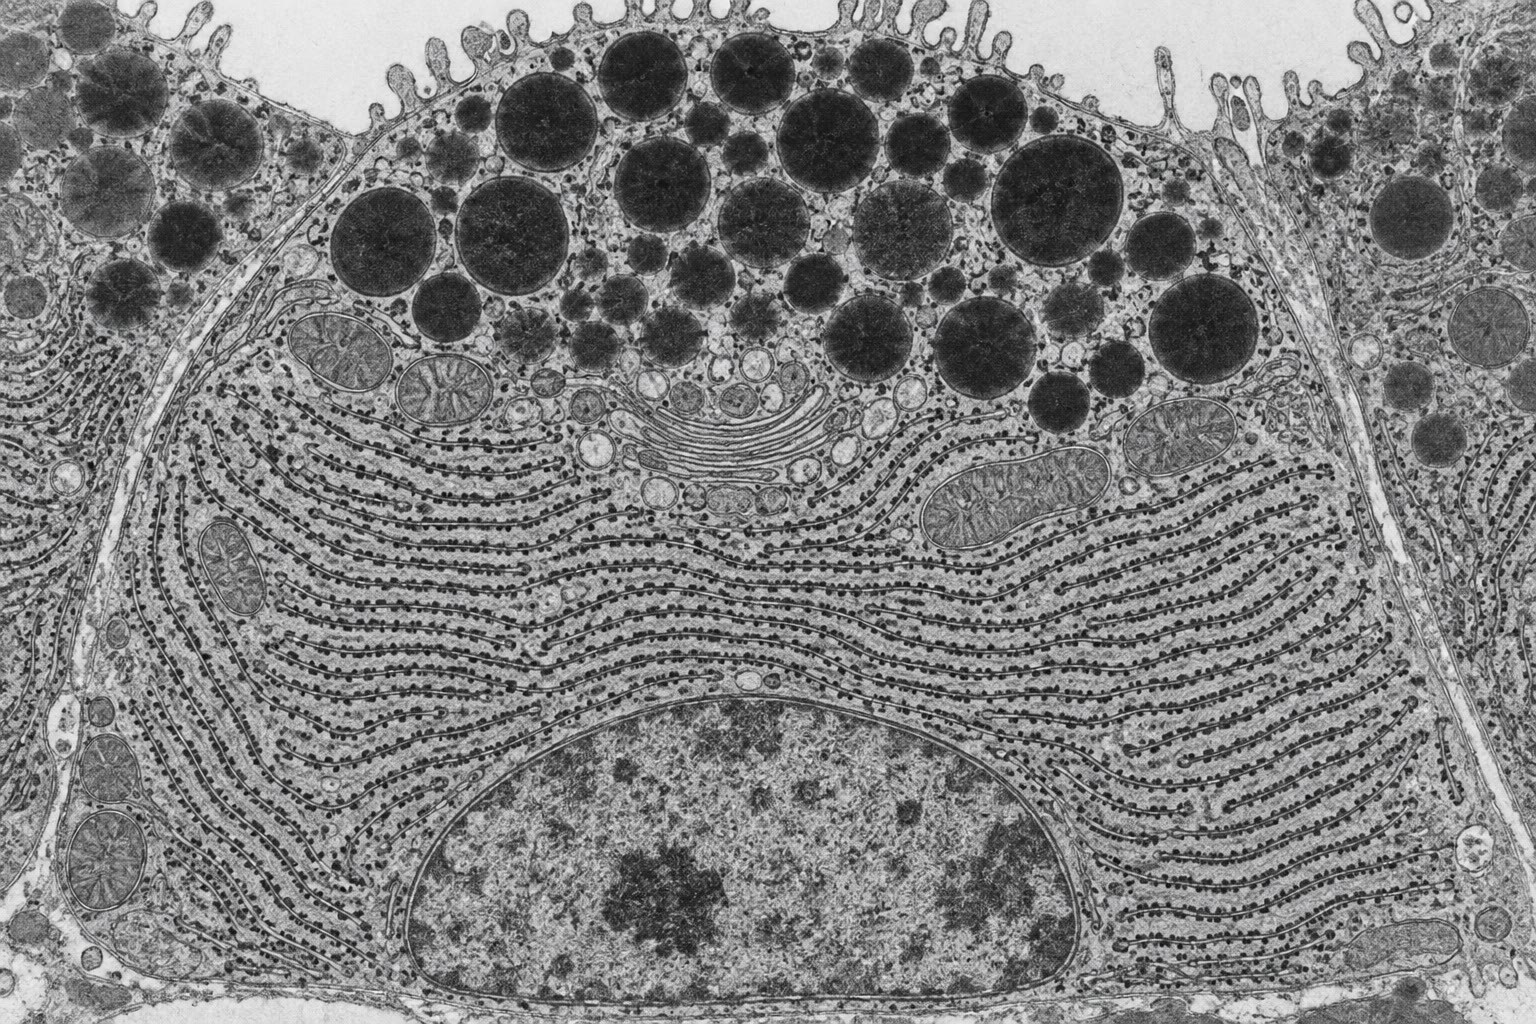
\includegraphics[width=0.56\linewidth]{images/book5/ai/b5-08-pancreas-acinar.jpg}

{\small Een acinaire cel van de alvleesklier in de
elektronenmicroscoop: gestapeld ruw endoplasmatisch reticulum, bezaaid
met ribosomen, vult de basis, het golgiapparaat ligt boven de kern, en
dichte secretiekorrels met verteringsenzym liggen opeengepakt onder het
apicale oppervlak, wachtend op een signaal.}
\end{omfigure}

\section{Blaasjes: knoppen, richten, versmelten}

\begin{definition}[Manteleiwitten en het knoppen van blaasjes]\label{def:b3:membrane-traffic:coats}
\index{bekleed blaasje}\index{COPII}\index{COPI}\index{clathrine}\index{klein GTPase}
Een transportblaasje wordt gevormd door een \emph{mantel} van eiwitten
die zich op de cytosolische kant van een membraan samenstelt, het
membraan tot een knop van \qtyrange{60}{100}{nm} kromt, vracht
verzamelt via receptoren die het membraan doorspannen, en wordt
afgeworpen zodra het blaasje is afgesnoerd. Drie mantels bedienen de
hoofdroutes: \emph{COPII} voor blaasjes die het reticulum naar het
golgiapparaat verlaten, \emph{COPI} voor het verkeer terug van het
golgiapparaat naar het reticulum en tussen de golgicisternen, en
\emph{clathrine} --- een driebenig eiwit dat tot een kooi van
zeshoeken en vijfhoeken polymeriseert --- voor blaasjes die het
trans-golginetwerk verlaten naar endosomen en voor de endocytose aan
het plasmamembraan, waar adaptoreiwitten de kooi aan de receptoren
koppelen die worden opgenomen. Elke mantel wordt aangetrokken door een
\emph{klein GTPase} (Sar1 voor COPII, Arf1 voor COPI en clathrine) dat
zich in zijn GTP-vorm in het membraan steekt en de mantel laat afvallen
zodra het na het knoppen GTP hydrolyseert. Terughaalsignalen houden de
compartimenten gescheiden: ontsnapte reticulumeiwitten met KDEL worden
in het golgiapparaat door een receptor gebonden en in COPI-blaasjes
teruggebracht.
\end{definition}

\begin{omfigure}
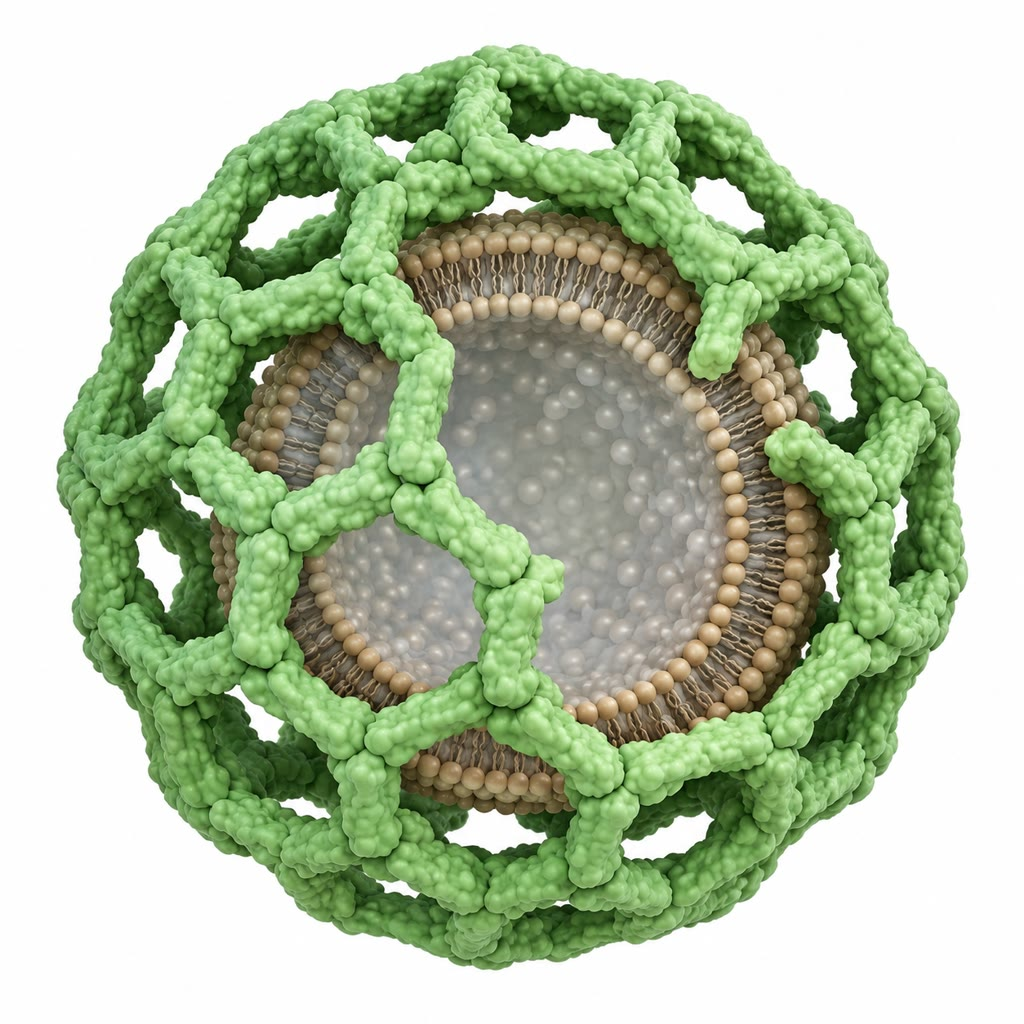
\includegraphics[width=0.36\linewidth]{images/book5/ai/b5-08-clathrin-cage.jpg}\hspace{0.04\linewidth}
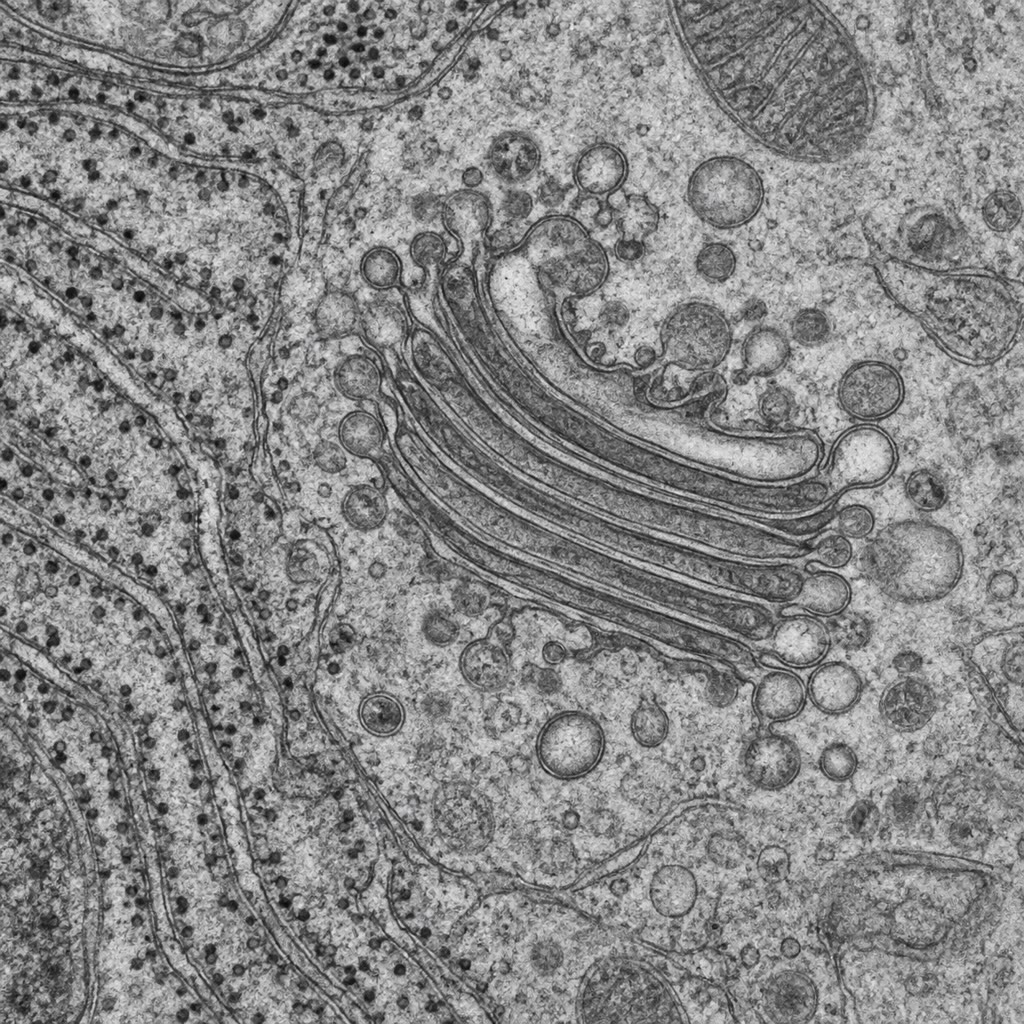
\includegraphics[width=0.36\linewidth]{images/book5/ai/b5-08-golgi-tem.jpg}

{\small Links: een clathrinekooi, het veelvlakkige rooster van
driebenige eenheden dat een endocytoseblaasje vorm geeft (opengesneden
om het membraan erbinnen te tonen). Rechts: een golgistapel in de
elektronenmicroscoop, een stapel afgeplatte cisternen met blaasjes die
van de randen knoppen.}
\end{omfigure}

\begin{definition}[Richten en versmelten]\label{def:b3:membrane-traffic:fusion}
\index{Rab-GTPase}\index{SNARE}\index{membraanfusie}\index{synaptotagmine}
Een blaasje vindt zijn doelwit met twee lagen herkenning. De
\emph{Rab-GTPasen} --- zo'n zestig in een menselijke cel, elk op de
membranen van één compartiment --- trekken lange touweiwitten aan die
een binnenkomend blaasje met het bijbehorende Rab vangen. Daarna
treden de \emph{SNAREs} op: een v-SNARE op het blaasje en t-SNAREs op
het doelwit, helicale eiwitten die in hun membranen zijn verankerd,
winden zich vanaf hun verre uiteinden naar de membranen toe om elkaar,
en de energie van de vierhelixbundel die zij vormen trekt de twee
dubbellagen naar elkaar toe tot zij versmelten. Elke SNARE-paring is
specifiek, een tweede controle op het adres. Na de fusie wordt de
bundel door het ATPase NSF weer uiteengewrikt voor hergebruik. De fusie
kan op een signaal worden laten wachten: in het zenuwuiteinde worden de
SNAREs half geritst vastgehouden door complexine tot
\emph{synaptotagmine}, dat het calcium bindt dat binnenkomt wanneer een
actiepotentiaal aankomt, het ritsen in minder dan een milliseconde
voltooit --- het vrijkomen van neurotransmitter dat in het boek van
jaar~2 is behandeld. De neurotoxinen van tetanus en botulisme zijn
proteasen die SNAREs knippen.
\end{definition}

\begin{proof}[Bewijsmateriaal]
Novick en Schekman (1980) isoleerden temperatuurgevoelige gistmutanten
die bij \qty{37}{\celsius} met uitscheiden ophielden en eiwit ophoopten
in het compartiment waar hun defect de weg versperde --- reticulum,
golgiapparaat of blaasjes opgestapeld onder het oppervlak; de $23$
\emph{sec}-genen bakenden de stappen af en bleken, eenmaal gekloneerd,
te coderen voor de \omterm{def:b3:membrane-traffic:coats}{mantels}, de GTPasen en de \omterm{def:b3:membrane-traffic:fusion}{SNAREs}. Rothman bouwde
het transport tussen golgicisternen na in een reageerbuis met
gezuiverde membranen, cytosol en ATP, en zuiverde daaruit NSF en de
\omterm{def:b3:membrane-traffic:fusion}{SNAREs}; de twee benaderingen kwamen op dezelfde eiwitten uit, en de
machinerie van gist en die van zoogdieren bleken dezelfde.
\end{proof}

\begin{omfigure}
\begin{tikzpicture}[every node/.style={font=\scriptsize}, >=stealth]
  % three stages left to right
  \foreach \x/\gap/\lab in {0/1.2/{1. vastgehouden door Rab}, 4.4/0.55/{2. SNAREs ritsen}, 8.8/0.0/{3. fusie, vracht vrij}} {
    % target membrane
    \draw[very thick, omDef] (\x,0) -- (\x+3.4,0); \draw[very thick, omDef] (\x,-0.3) -- (\x+3.4,-0.3);
    \node[below, align=center] at (\x+1.7,-0.45) {\lab};
  }
  % stage 1 vesicle
  \draw[very thick, omProp] (1.7,1.2+0.8) circle (0.8); \draw[very thick, omProp] (1.7,1.2+0.8) circle (0.6);
  \draw[omThm, thick] (1.4,1.25) -- (1.4,0.35); \draw[omThm, thick] (2.0,1.25) -- (2.0,0.35);
  \draw[omMeth!70!black, thick] (1.7,1.2) -- (1.7,0.6); \draw[omMeth!70!black, thick] (1.7,0.6) -- (1.7,0.0);
  \draw[thick, fill=omExo!40] (0.7,0.9) ellipse (0.25 and 0.2); \node[left] at (0.45,0.9) {Rab};
  \draw[thick, omExo!70!black] (0.95,0.9) .. controls (1.1,0.5) .. (1.2,0.05); \node[left, font=\tiny] at (0.9,0.4) {touw};
  \node[right, font=\tiny] at (2.05,0.8) {SNAREs};
  % stage 2 vesicle closer, helices twisted
  \draw[very thick, omProp] (6.1,0.55+0.8) circle (0.8); \draw[very thick, omProp] (6.1,0.55+0.8) circle (0.6);
  \draw[omThm, very thick] (5.85,0.6) .. controls (6.2,0.5) and (5.9,0.3) .. (6.1,0.05);
  \draw[omMeth!70!black, very thick] (6.35,0.6) .. controls (6.0,0.5) and (6.3,0.3) .. (6.1,0.05);
  \node[right, font=\tiny, align=left] at (6.6,0.35) {de vierhelixbundel\\trekt de membranen\\naar elkaar toe};
  % stage 3 fused omega shape
  \draw[very thick, omProp] (9.7,0) .. controls (9.7,1.5) and (11.3,1.5) .. (11.3,0);
  \draw[very thick, omProp] (9.9,-0.3) .. controls (9.9,1.1) and (11.1,1.1) .. (11.1,-0.3);
  \foreach \p in {(10.5,-0.9),(10.2,-1.1),(10.8,-1.15)} \fill[omExo] \p circle (0.06);
  \draw[->, omExo, thick] (10.5,0.5) -- (10.5,-0.6);
  \node[right, font=\tiny, align=left] at (11.4,0.8) {NSF ritst de\\SNAREs later\\weer los};
\end{tikzpicture}

{\small Fusie in drie stappen. Een Rab op het blaasje en een touw op
het doelwit brengen de twee membranen binnen bereik; de \omterm{def:b3:membrane-traffic:fusion}{SNAREs} van
blaasje en doelwit (rood en groen) ritsen tot een vierhelixbundel die
de dubbellagen naar elkaar toe sleept; zij versmelten en de vracht komt
het doelcompartiment binnen.}
\end{omfigure}

\begin{proposition}[Het golgiapparaat]\label{prop:b3:membrane-traffic:golgi}
\index{golgiapparaat}\index{cisternerijping}\index{mannose-6-fosfaat}
Het golgiapparaat is een stapel van vier tot acht afgeplatte cisternen,
met de cis-zijde naar het reticulum en de trans-zijde naar het
plasmamembraan, waarbij elke cisterne een andere reeks enzymen herbergt
die de suikers van passerende glycoproteïnen bijknippen en opnieuw
opbouwen en die O-gebonden suikers, sulfaat en fosfaat toevoegen. De
vracht schuift vooral op door \emph{\omterm{prop:b3:membrane-traffic:golgi}{cisternerijping}}: aan de cis-zijde
ontstaat uit aankomende blaasjes een nieuwe cisterne, die net als de
cisternen vóór haar door de stapel beweegt en rijpt terwijl
COPI-blaasjes de enzymen van elke cisterne achterwaarts naar de jongere
erachter brengen; aan de trans-zijde valt zij uiteen in blaasjes die
naar hun bestemming vertrekken. Daar wordt het sorteren beslist:
lysosomale hydrolasen, in het cis-golgiapparaat gemerkt met
\emph{mannose-6-fosfaat}, worden door hun receptor gebonden en in
clathrineblaasjes voor het \omterm{def:b3:membrane-traffic:endocytosis}{endosoom} verpakt; gereguleerde
secretie-eiwitten klonteren bij de licht zure pH samen tot
condenserende korrels; al het overige vertrekt in de constitutieve
stroom naar het oppervlak. Bij de I-celziekte ontbreekt het
fosforylerende enzym, worden de hydrolasen uitgescheiden in plaats van
afgeleverd, en lopen de lysosomen vol onverteerd materiaal.
\end{proposition}

\begin{omfigure}
\begin{tikzpicture}[every node/.style={font=\scriptsize}, >=stealth]
  % plasma membrane top
  \draw[very thick, omDef] (0,4.2) -- (12,4.2); \node[above] at (6,4.25) {plasmamembraan \quad (buiten erboven)};
  % ER
  \draw[thick, fill=omDef!12] (0.3,0.0) rectangle (4.0,0.9); \node at (2.15,0.45) {endoplasmatisch reticulum};
  % Golgi stack
  \foreach \y in {1.5,1.85,2.2,2.55} \draw[thick, fill=omProp!25] (4.8,\y) ellipse (1.4 and 0.13);
  \node[right] at (6.3,1.5) {cis}; \node[left] at (3.35,2.55) {trans};
  \node[right] at (6.3,2.05) {golgistapel};
  % ER -> Golgi (COPII)
  \draw[->, thick, omMeth!70!black] (3.9,0.95) -- (4.5,1.4); \node[right, omMeth!70!black, font=\tiny] at (4.35,1.02) {COPII};
  % Golgi -> ER (COPI)
  \draw[->, thick, omThm] (3.6,1.42) -- (2.9,0.95); \node[left, omThm, font=\tiny] at (2.95,1.3) {COPI, KDEL-terughaling};
  % trans Golgi -> PM constitutive
  \draw[->, thick, omMeth!70!black] (5.6,2.7) -- (7.6,4.1); \node[left, font=\tiny, align=right] at (6.4,3.6) {constitutieve\\secretie};
  % trans -> secretory granule -> PM regulated
  \draw[->, thick, omMeth!70!black] (4.6,2.7) -- (4.0,3.3); \draw[thick, fill=omExo!50] (3.8,3.5) circle (0.22); \draw[->, thick, omMeth!70!black] (3.8,3.75) -- (3.8,4.1);
  \node[left, font=\tiny, align=right] at (3.55,3.5) {secretiekorrel:\\gereguleerd, op een signaal};
  % trans -> endosome/lysosome (clathrin, M6P)
  \draw[->, thick, omProp!80!black] (6.0,2.62) -- (8.25,2.62); \node[above, font=\tiny] at (7.1,2.67) {clathrine, M6P-receptor};
  \draw[thick, fill=omProp!20] (8.8,2.7) circle (0.5); \node at (8.8,2.7) {\tiny endosoom};
  \draw[->, thick, omProp!80!black] (9.25,2.4) -- (10.2,1.95); \draw[thick, fill=omThm!25] (10.7,1.6) circle (0.5); \node at (10.7,1.6) {\tiny lysosoom};
  % endocytosis from PM to endosome
  \draw[->, thick, omDef] (9.6,4.15) -- (9.1,3.2); \node[right, font=\tiny, align=left] at (9.5,3.7) {endocytose\\(clathrineputjes)};
  % recycling endosome -> PM
  \draw[->, thick, omDef] (8.5,3.2) -- (8.0,4.15); \node[left, font=\tiny] at (8.3,3.3) {recycling};
  % lysosome inputs autophagy
  \draw[->, thick, gray] (11.9,0.6) -- (11.1,1.3); \node[below, font=\tiny, align=center] at (11.9,0.55) {autofagosoom\\(cytoplasma, organellen)};
\end{tikzpicture}

{\small De kaart van het membraanverkeer. Naar buiten (groen): van het
reticulum naar het golgiapparaat in COPII-blaasjes, van het
golgiapparaat naar het oppervlak, hetzij constitutief hetzij via
korrels die op een signaal wachten. Terug (rood): COPI-blaasjes brengen
ontsnapte reticulumeiwitten terug. Omlaag (oranje): lysosomale enzymen
gemerkt met mannose-6-fosfaat gaan naar het \omterm{def:b3:membrane-traffic:endocytosis}{endosoom} en het \omterm{def:b3:membrane-traffic:endocytosis}{lysosoom}.
Naar binnen (blauw): endocytose vanaf het oppervlak, met de meeste
receptoren gerecycled.}
\end{omfigure}

\section{Endocytose en het lysosoom}

\begin{definition}[Endocytose]\label{def:b3:membrane-traffic:endocytosis}
\index{receptorgemedieerde endocytose}\index{endosoom}\index{lysosoom}\index{autofagie}
De \emph{receptorgemedieerde endocytose} concentreert een ligand dat
aan oppervlaktereceptoren is gebonden in met \omterm{def:b3:membrane-traffic:coats}{clathrine} beklede putjes,
die zich afsnoeren (het GTPase dynamine snoert de hals dicht) als
blaasjes van ongeveer \qty{100}{nm} --- duizend per minuut in een
fibroblast, wat het hele oppervlaktemembraan in een uur omzet. De
blaasjes versmelten tot \emph{vroege endosomen}, waarvan het lumen door
een protonpomp tot pH~6 wordt aangezuurd; de meeste liganden laten hun
receptoren daar los, de receptoren keren in recyclingblaasjes terug
naar het oppervlak, en het ligand reist verder terwijl het endosoom tot
laat endosoom rijpt (pH~5,5) en met een \emph{lysosoom} versmelt: een
compartiment bij pH~4,5--5 met zo'n zestig hydrolasen --- proteasen,
nucleasen, lipasen, glycosidasen --- die alleen bij die pH werken,
zodat een lek in het neutrale cytosol weinig schade doet. Het lysosoom
verteert ook het eigen materiaal van de cel, dat door \emph{autofagie}
wordt aangeleverd: een dubbel membraan groeit om een stuk cytoplasma of
een versleten organel heen, sluit zich tot een autofagosoom en
versmelt met het lysosoom; de producten gaan terug naar het cytosol. De
autofagie wordt aangezet door uithongering (zij hergebruikt de eigen
stof van een cel voor energie) en ruimt klonters en beschadigde
mitochondriën op; haar falen wordt met neurodegeneratie in verband
gebracht.
\end{definition}

\begin{proof}[Bewijsmateriaal]
Brown en Goldstein (jaren zeventig) volgden het lipoproteïne met lage
dichtheid (LDL), het deeltje dat cholesterol in het bloed vervoert, in
gekweekte fibroblasten. LDL bond verzadigbaar aan zo'n \num{20000}
plaatsen per cel aan het oppervlak, werd binnen minuten in beklede
putjes opgenomen, en zijn cholesterol kwam in de lysosomen vrij en zette
de eigen cholesterolsynthese van de cel uit. Fibroblasten van patiënten
met familiaire hypercholesterolemie bonden geen LDL (receptor afwezig)
of bonden het wel maar namen het niet op (een mutatie in de
cytosolische staart van de receptor die belet dat clathrine-adaptoren
hem vangen): de ziekte was een defect van de endocytose, de staart van
de receptor bevatte het opnamesignaal, en de recyclende receptor ---
die elk honderden rondreizen maakt --- werd als het algemene mechanisme
van opname vastgesteld.
\end{proof}

\begin{proposition}[Opname via recyclende receptoren]\label{prop:b3:membrane-traffic:uptake}
\index{receptorrecycling}
Laat een cel in totaal $R$ receptoren hebben, waarvan $S$ aan het
oppervlak en $R - S$ binnenin op de terugweg. Een receptor aan het
oppervlak is bezet met kans $\theta = [L]/(K_{d} + [L])$, een bezette
receptor wordt met snelheid $k_{i}$ opgenomen, en een opgenomen
receptor keert terug met snelheid $k_{r}$. In evenwicht is de
ligandstroom de cel in
\[
J = \frac{R\,k_{i}k_{r}\,\theta}{k_{r} + k_{i}\theta},
\]
die bij stijgende ligandconcentratie verzadigt bij $J_{\max} =
R\,k_{i}k_{r}/(k_{i} + k_{r})$: de opname van een cel wordt niet alleen
begrensd door haar receptoren maar door hoe snel zij die kan
terughalen.
\end{proposition}
\begin{proof}
Receptoren aan het oppervlak gaan verloren met snelheid $k_{i}\theta S$
en komen terug met snelheid $k_{r}(R - S)$; in evenwicht heffen die
elkaar op, dus $S = R\,k_{r}/(k_{r}
+ k_{i}\theta)$. Elke opname voert één ligand mee, dus $J =
k_{i}\theta S$, wat de formule geeft. Voor $\theta \to 1$ nadert de
stroom $R\,k_{i}k_{r}/(k_{r} + k_{i})$ --- de receptoren draaien zo snel
rond als de twee snelheden toelaten, met een deel $k_{r}/(k_{i} + k_{r})$
op elk moment aan het oppervlak.
\end{proof}

\begin{example}[Cholesterol per deeltje]\label{ex:b3:membrane-traffic:ldl}
Een fibroblast met $R = \num{20000}$ LDL-receptoren, een opnametijd van
\qty{5}{min} ($k_{i} = \qty{0.2}{min^{-1}}$) en een terugkeertijd van
\qty{10}{min} ($k_{r} = \qty{0.1}{min^{-1}}$) neemt bij verzadigend LDL
$J_{\max} = \num{20000}\times 0.2\times 0.1/0.3 \approx 1300$ deeltjes
per minuut op, met op elk moment een derde van zijn receptoren aan het
oppervlak; elk deeltje brengt zo'n \num{1500} moleculen cholesterol,
twee miljoen per minuut, genoeg om ongeveer een tiende vierkante
micrometer membraan te bouwen. Een heterozygoot voor familiaire
hypercholesterolemie, met de helft van de receptoren, neemt half zoveel
op; het bloedcholesterol verdubbelt en de hartziekte komt twintig jaar
te vroeg. De statines verhogen $R$ door de levercel van haar eigen
cholesterol te beroven.
\end{example}

\begin{omfigure}
\begin{tikzpicture}
\begin{axis}[
  width=0.7\linewidth, height=5.4cm,
  axis x line=bottom, axis y line=left,
  xmin=0, xmax=10, ymin=0, ymax=1500,
  xlabel={LDL-concentratie, $[L]/K_{d}$}, ylabel={deeltjes per minuut},
  xlabel style={font=\small, at={(axis description cs:0.5,-0.12)}, anchor=north},
  ylabel style={font=\small},
  tick label style={font=\small}, xtick={0,2,4,6,8,10}, ytick={0,500,1000,1333}, yticklabels={0,500,1000,$J_{\max}$},
  clip=false,
]
\addplot[very thick, omDef, domain=0:10, samples=60] {20000*0.2*0.1*(x/(1+x))/(0.1+0.2*(x/(1+x)))};
\addplot[very thick, omThm, domain=0:10, samples=60] {10000*0.2*0.1*(x/(1+x))/(0.1+0.2*(x/(1+x)))};
\addplot[dashed, gray, domain=0:10, samples=2] {1333};
\node[font=\scriptsize, omDef, anchor=north west] at (axis cs:4,900) {$R = \num{20000}$};
\node[font=\scriptsize, omThm, anchor=north west] at (axis cs:4,560) {$R = \num{10000}$ (heterozygoot)};
\end{axis}
\end{tikzpicture}

{\small Opname van LDL via recyclende receptoren, met de formule van de
propositie en $k_{i} = \qty{0.2}{min^{-1}}$ en $k_{r} =
\qty{0.1}{min^{-1}}$: verzadigend met ligand, en gehalveerd wanneer de
helft van de receptoren ontbreekt.}
\end{omfigure}

\begin{remark}[Eén membraan, vele compartimenten]\label{rem:b3:membrane-traffic:one-membrane}
Elk membraan van het secretie- en endocytosesysteem is topologisch
gezien één membraan: het lumen van het reticulum is via blaasjes
doorlopend verbonden met de buitenkant van de cel, en een lipide of
eiwit dat in het reticulum wordt gemaakt kan het oppervlak bereiken
zonder ooit een dubbellaag over te steken. Wat de compartimenten
gescheiden houdt zijn geen wanden maar verkeer --- selectief inpakken
naar buiten, selectief terughalen naar binnen, en bij elke fusie een
bepaald paar herkenningsmoleculen. De compartimenten zijn
evenwichtstoestanden van stromen, als de kolken van een rivier, en een
cel die het verkeer stillegt verliest haar geografie binnen enkele
uren.
\end{remark}

\section{Opgaven}

\begin{exercise}[$\star$]\label{exo:b3:membrane-traffic:1}
Geef bij elk het signaal en de bestemming: een stuk van twintig
hydrofobe residuen aan de aminoterminus; PKKKRKV; een amfipathische
aminoterminale helix; KDEL aan de carboxyterminus; een
mannose-6-fosfaat op de suikers.
\end{exercise}

\begin{exercise}[$\star$]\label{exo:b3:membrane-traffic:2}
Beschrijf de drie belangrijkste waarnemingen van het experiment van
Blobel en Dobberstein en wat elk ervan aantoonde.
\end{exercise}

\begin{exercise}[$\star$]\label{exo:b3:membrane-traffic:3}
Noem de \omterm{def:b3:membrane-traffic:coats}{mantel} en de richting van het transport voor: reticulum naar
golgiapparaat; golgiapparaat naar reticulum; trans-golginetwerk naar
\omterm{def:b3:membrane-traffic:endocytosis}{endosoom}; plasmamembraan naar \omterm{def:b3:membrane-traffic:endocytosis}{endosoom}.
\end{exercise}

\begin{exercise}[$\star$]\label{exo:b3:membrane-traffic:4}
Waarom zitten de suikers van een eiwit in het plasmamembraan altijd aan
de buitenkant van de cel?
\end{exercise}

\begin{exercise}[$\star\star$]\label{exo:b3:membrane-traffic:5}
Bepaal in het model van \cref{thm:b3:membrane-traffic:pulse-chase} met
$k_{1}
= \qty{0.2}{min^{-1}}$ en $k_{2} = \qty{0.05}{min^{-1}}$ wanneer het
merkstof in het golgiapparaat zijn maximum bereikt en hoeveel er dan
zit; daarna het deel in de korrels na \qty{60}{min}.
\end{exercise}

\begin{exercise}[$\star\star$]\label{exo:b3:membrane-traffic:6}
Een membraaneiwit heeft hydrofobe stukken van $22$ residuen op de
posities 30, 90, 150 en 210 en een aminoterminaal \omterm{def:b3:membrane-traffic:signals}{signaalpeptide}. Teken
of beschrijf zijn topologie: hoeveel helices, en naar welke kant elk
segment ertussen wijst. Waar kan het worden geglycosyleerd?
\end{exercise}

\begin{exercise}[$\star\star$]\label{exo:b3:membrane-traffic:7}
Bereken met \cref{prop:b3:membrane-traffic:uptake} bij $R = \num{30000}$,
$k_{i} = \qty{0.25}{min^{-1}}$ en $k_{r} = \qty{0.05}{min^{-1}}$ de
waarde van $J_{\max}$ en het deel van de receptoren dat bij verzadiging
aan het oppervlak zit. Welke enkele verandering zou de opname
verdubbelen?
\end{exercise}

\begin{exercise}[$\star\star$]\label{exo:b3:membrane-traffic:8}
Voorspel het lot van de lysosomale hydrolasen, en het fenotype, in (a)
een cel zonder de mannose-6-fosfaatreceptor, (b) een cel zonder het
fosfotransferase dat het merkteken aanbrengt, (c) een cel behandeld met
een middel dat de pH van het \omterm{def:b3:membrane-traffic:endocytosis}{endosoom} neutraliseert.
\end{exercise}

\begin{exercise}[$\star\star$]\label{exo:b3:membrane-traffic:9}
De JD-mutatie in de LDL-receptor verandert een tyrosine in de
cytosolische staart. Cellen die LDL normaal binden nemen het niet op.
Verklaar het mechanisme, en voorspel waar de receptoren op het
celoppervlak liggen ten opzichte van de beklede putjes.
\end{exercise}

\begin{exercise}[$\star\star\star$]\label{exo:b3:membrane-traffic:10}
Los het pulsmodel op voor het geval $k_{1} = k_{2} = k$ (de formule van
de stelling is daar singulier): laat zien dat $B(t) = kt\,e^{-kt}$ en
zoek het maximum. Leg daarna uit waarom het meten van alleen het
korreldeel $C(t)$ de twee snelheden niet afzonderlijk kan bepalen.
\end{exercise}

\begin{exercise}[$\star\star\star$]\label{exo:b3:membrane-traffic:11}
Een fibroblast neemt per minuut \num{1000} clathrineblaasjes met een
diameter van \qty{100}{nm} op en heeft een oppervlak van
\qty{3000}{\micro m^2}. Hoe lang duurt het om het equivalent van het
hele oppervlak op te nemen? Waarom krimpt de cel niet, en wat zegt de
balans over de snelheid van de exocytose en over het volume vloeistof
dat per uur wordt opgenomen?
\end{exercise}

\begin{exercise}[$\star\star\star$]\label{exo:b3:membrane-traffic:12}
Botulinetoxine knipt een \omterm{def:b3:membrane-traffic:fusion}{SNARE} in motorische zenuwuiteinden;
tetanustoxine knipt dezelfde \omterm{def:b3:membrane-traffic:fusion}{SNARE} in remmende schakelneuronen van het
ruggenmerg. Leg uit waarom het eerste een slappe en het tweede een
krampachtige verlamming veroorzaakt, en waarom een toxine dat de fusie
blokkeert in de geneeskunde bij minieme doses nuttig is.
\end{exercise}

\section{Vraagstuk: een dag van een alvleeskliercel}

\begin{problem}[{Weekendvraagstuk --- de doorvoer van een secretiecel
geteld in moleculen, blaasjes en vierkante micrometers, haar
pulscurven opgelost, de cholesterolopname van een levercel berekend via
recyclende receptoren, en een lysosoom proton voor proton aangezuurd,
met als besluit het tijdstip van het golgimaximum, het aantal blaasjes
dat per minuut knopt en het aantal LDL-deeltjes dat per uur wordt
opgenomen}]
\label{pb:b3:membrane-traffic:1}
Gegevens: een acinaire cel maakt $10^{7}$ enzymmoleculen per minuut,
elk \qty{25}{kDa} en \qty{4}{nm} groot. Transportblaasjes zijn bollen
met een diameter van \qty{70}{nm}; een korrel is een bol van
\qty{1}{\micro m}. Membraanoppervlak per lipidemolecuul
\qty{0.7}{nm^2}, twee lagen. Het reticulum van de cel heeft een
oppervlak van \qty{6000}{\micro m^2}. Puls en jacht:
$k_{1} = \qty{0.1}{min^{-1}}$, $k_{2} = \qty{0.05}{min^{-1}}$. Een
levercel: $R = \num{50000}$ LDL-receptoren, $k_{i} = \qty{0.2}{min^{-1}}$,
$k_{r} = \qty{0.1}{min^{-1}}$, $K_{d} = \qty{2}{nmol/L}$, LDL-concentratie
in het plasma \qty{2}{nmol/L}; \num{1500} cholesterolmoleculen
per deeltje.
Een \omterm{def:b3:membrane-traffic:endocytosis}{lysosoom}: bol van \qty{0.5}{\micro m}, pH van $7.2$ naar $4.7$, met
een buffercapaciteit zodanig dat er $50$ protonen moeten worden gepompt
voor elk proton dat vrij blijft; een protonpomp verzet $200$ protonen
per seconde.

\medskip
\noindent\textbf{Deel I --- Doorvoer.}
\begin{enumerate}
  \item Welke massa enzym maakt de cel per minuut, en per dag?
        Vergelijk met haar eigen eiwitgehalte van ongeveer
        \qty{300}{pg}.
  \item Hoeveel enzymmoleculen passen er in een blaasje als zij
        \qty{30}{\%} van het volume vullen (bol van \qty{4}{nm})?
        Hoeveel blaasjes verlaten het reticulum per minuut?
  \item Hoeveel membraanoppervlak voeren die blaasjes per minuut mee,
        en in hoeveel tijd zouden zij het hele reticulum opgebruiken
        als er niets terugkwam?
  \item Hoeveel lipidemoleculen is dat per minuut? Wat moet de cel doen
        om haar reticulum te behouden?
  \item Hoeveel enzymmoleculen passen er bij dezelfde pakking in een
        korrel, en hoeveel korrels vult de cel per uur?
  \item Een maaltijd leegt $300$ korrels in tien minuten door fusie met
        het apicale membraan, waarbij hun membraan wordt toegevoegd aan
        een oppervlak van \qty{50}{\micro m^2}. Met welke factor groeit
        het apicale oppervlak, en wat moet daarop volgen?
\end{enumerate}

\medskip
\noindent\textbf{Deel II --- Timing.}
\begin{enumerate}[resume]
  \item Wanneer bereikt het merkstof in het golgiapparaat met de
        gegeven snelheden zijn maximum, en welk deel zit daar dan?
  \item Welk deel van een puls zit na \qty{30}{min} in het reticulum,
        het golgiapparaat en de korrels?
  \item Wat zijn de gemiddelde verblijfstijden in de twee
        compartimenten? Wat is de gemiddelde totale tijd van synthese
        tot korrel?
  \item Een geneesmiddel vertraagt het vertrek uit het golgiapparaat
        tot $k_{2} = \qty{0.01}{min^{-1}}$. Wat zijn het nieuwe
        tijdstip en het nieuwe maximum; hoe ziet het golgiapparaat er
        in de microscoop uit?
  \item Leg uit waarom het maximale golgideel $k_{1}/k_{2}$ tot een
        macht is (geef de macht) en daarom altijd onder $1$ ligt.
  \item Wat zou $B(t)$ naderen als de reticulumstap veel sneller was
        dan de golgistap? Geef de betekenis.
\end{enumerate}

\medskip
\noindent\textbf{Deel III --- Cholesterol.}
\begin{enumerate}[resume]
  \item Bereken $\theta$ bij de LDL-concentratie in het plasma, en de
        opname $J$ in deeltjes per minuut en per uur.
  \item Hoeveel cholesterolmoleculen per uur? De membranen van de cel
        bevatten $5\times 10^{9}$ cholesterolmoleculen; hoe lang duurt
        het om ze alle uit LDL alleen te vervangen?
  \item Bereken het deel van de receptoren aan het oppervlak en het
        aantal rondreizen dat elke receptor in zijn levensduur van
        \qty{20}{h} maakt.
  \item Een heterozygoot heeft $R = \num{25000}$: herbereken $J$. Het
        LDL in het plasma stijgt tot de opname de aanmaak evenaart: met
        welke factor, als $\theta$ ruim onder de verzadiging ligt?
  \item Een statine verdubbelt $R$ in de levercellen van de
        heterozygoot. Wat gebeurt er volgens dezelfde redenering met
        het LDL in het plasma?
  \item Leg uit waarom de homozygoot zonder receptoren, met vijf keer
        het normale LDL in het plasma, er toch slechter aan toe is dan
        de rekenkunde van vraag 16 alleen doet vermoeden.
\end{enumerate}

\medskip
\noindent\textbf{Deel IV --- Zuur.}
\begin{enumerate}[resume]
  \item Bereken het volume van het \omterm{def:b3:membrane-traffic:endocytosis}{lysosoom} in liters en het aantal
        vrije protonen bij pH $7.2$ en bij pH $4.7$.
  \item Hoeveel protonen moeten er met de buffering in totaal worden
        gepompt? Hoe lang duurt dat met $50$ pompen?
  \item De pomp verzet protonen tegen de gradiënt in. Welk elektrisch
        probleem ontstaat daarbij, en hoe wordt het opgelost (denk aan
        een tegenion)?
  \item Waarom zijn de hydrolasen pas bij pH~5 werkzaam, en wat
        beschermt dat?
  \item Waarom laat de LDL-receptor LDL los bij pH~6, terwijl de
        mannose-6-fosfaatreceptor zijn vracht bij dezelfde pH loslaat
        --- wat moeten beide eiwitten gemeen hebben?
  \item Chloroquine is een zwakke base die ongeladen membranen
        oversteekt en gevangen raakt zodra zij is geprotoneerd. Met
        welke factor hoopt zij zich op in een \omterm{def:b3:membrane-traffic:endocytosis}{lysosoom} bij pH $4.7$ ten
        opzichte van het cytosol bij pH $7.2$ (de verhouding van de
        protonconcentraties), en wat doet dat met het \omterm{def:b3:membrane-traffic:endocytosis}{lysosoom}?
  \item Vat samen: het tijdstip van het golgimaximum (vraag~7), het
        aantal blaasjes dat per minuut het reticulum verlaat (vraag~2),
        en het aantal LDL-deeltjes dat per uur wordt opgenomen
        (vraag~13).
\end{enumerate}
\end{problem}
